\begin{center}
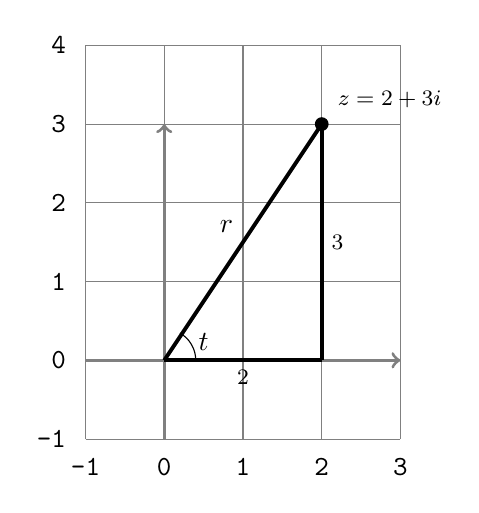
\begin{tikzpicture}
\draw[gray] (-1,-1) to  (-1,4);
\draw[gray] (0,-1) to  (0,4);
\draw[gray] (1,-1) to  (1,4);
\draw[gray] (2,-1) to  (2,4);
\draw[gray] (3,-1) to  (3,4);
\draw[gray] (-1,-1) to  (3,-1);
\draw[gray] (-1,0) to  (3,0);
\draw[gray] (-1,1) to  (3,1);
\draw[gray] (-1,2) to  (3,2);
\draw[gray] (-1,3) to  (3,3);
\draw[gray] (-1,4) to  (3,4);
\draw(-1, -1) node [font=\ttfamily, label=below:{\normalsize {\texttt{-1}}}] {};
\draw(0, -1) node [font=\ttfamily, label=below:{\normalsize {\texttt{0}}}] {};
\draw(1, -1) node [font=\ttfamily, label=below:{\normalsize {\texttt{1}}}] {};
\draw(2, -1) node [font=\ttfamily, label=below:{\normalsize {\texttt{2}}}] {};
\draw(3, -1) node [font=\ttfamily, label=below:{\normalsize {\texttt{3}}}] {};
\draw(-1, -1) node [font=\ttfamily, label=left:{\normalsize {\texttt{-1}}}] {};
\draw(-1, 0) node [font=\ttfamily, label=left:{\normalsize {\texttt{0}}}] {};
\draw(-1, 1) node [font=\ttfamily, label=left:{\normalsize {\texttt{1}}}] {};
\draw(-1, 2) node [font=\ttfamily, label=left:{\normalsize {\texttt{2}}}] {};
\draw(-1, 3) node [font=\ttfamily, label=left:{\normalsize {\texttt{3}}}] {};
\draw(-1, 4) node [font=\ttfamily, label=left:{\normalsize {\texttt{4}}}] {};
\draw[line width=0.04cm,black!50,->] (-1,0) to  (3,0);
\draw[line width=0.04cm,black!50,->] (0,-1) to  (0,3);

\fill[black] (2.0, 3.0) circle (0.08);
\draw[black] (2.0, 3.0) circle (0.08);
\node[anchor=south west] at (2.08,3.08)   {\footnotesize{$z = 2 + 3i$}};
\draw[line width=0.05cm,black] (0,0) to  (2,3);

\node[anchor=south east] at (1.0,1.5)   {$\footnotesize{r}$};
\draw[line width=0.05cm,black] (0,0) to  (2,0);

\node[anchor=north] at (1.0,0)   {\footnotesize{2}};
\draw[line width=0.05cm,black] (2,0) to  (2,3);

\node[anchor=west] at (2,1.5)   {\footnotesize{$3$}};
\draw[] (0.4,0) arc (0:60:0.4);
\node[anchor=south] at (0.5,0)   {{$t$}};
\end{tikzpicture}

\end{center}

